\documentclass[a4paper, 12pt]{article}
\usepackage{amsmath}
\usepackage{tkz-euclide}
\usepackage{tikz}
\usepackage{circuitikz}
\usepackage{amssymb}
\usepackage{pgfplots}
\pgfplotsset{compat=1.18}
\tikzset{european}
\title{Trigonometry}
\author{Hertzberg, Joakim D.}
\date{\today}
\begin{document}

%END OF PREAMBLE
\begin{titlepage}
\clearpage\maketitle
\begin{center}
MAT03c: Mathematics 3c
\end{center}
\thispagestyle{empty}
\end{titlepage}



\section{Trigonometric Functions}


\subsection{The \emph{sin} \& \emph{cos} functions}


The $\sin$ function is defined as \emph{the ratio between the opposite side and hypotenuse of a right angle triangle, at a certain angle $\theta$}. The $\cos$ function, on the other hand is defined as \emph{the ratio between the adjacent side and hypotenuse in a right triangle, defined at a certain angle $\theta$.}

%Fig. 1
\begin{figure}
\begin{center}
\begin{tikzpicture}[scale=2.0]
	
	\tkzDefPoint(0,0){C}
	\tkzDefPoint(4,0){B}
	\tkzDefPoint(4,3){A}

	\tkzLabelPoints(B, C)
	\tkzLabelPoints[above](A)

	\tkzDrawPolygon[thick](A,B,C)

	\tkzMarkRightAngle(C,B,A)

	\tkzLabelAngle[pos=1.25](B,C,A){$\theta$}
	\tkzMarkAngle(B,C,A)

	\tkzLabelLine[pos=0.5, above](C,A){b}
	\tkzLabelLine[pos=0.5, right](A,B){c}
	\tkzLabelLine[pos=0.5, below](C,B){a}
\end{tikzpicture}
\end{center}
\caption{A right angle triangle $\triangle ABC$}
\label{fig:tri1}
\end{figure} \bigbreak



In the above example, $\sin(\theta)$ is defined as follows: $$\sin(\theta) = \frac{c}{b}$$
And $\cos(\theta)$ as such: $$\cos(\theta) = \frac{a}{b}$$

\subsubsection{The Law of Sines}
\begin{center}
\begin{tikzpicture}[scale=2.0]
	\tkzDefPoint(0,0){A}
	\tkzDefPoint(4,0){B}
	\tkzDefPoint(3,2){C}
	\tkzDrawPolygon(A,B,C)


	\tkzMarkAngle[scale=0.75](B,A,C)
	\tkzLabelAngle[right, pos=0.6](B,A,C){A}

	\tkzMarkAngle[scale=0.75](A,C,B)
	\tkzLabelAngle[below, pos=0.6](A,C,B){C}

	\tkzMarkAngle[scale=0.75](C,B,A)
	\tkzLabelAngle[left, pos=0.6](C,B,A){B}


	%LINES

	\tkzLabelLine[pos=0.5, below](A,B){c}
	\tkzLabelLine[pos=0.5, right](C,B){a}
	\tkzLabelLine[pos=0.5, above](A,C){b}
\end{tikzpicture} \bigbreak


For this triangle it is true that:
\end{center}
$$\frac{\sin{A}}{a} \ = \ \frac{\sin{B}}{b} \ = \ \frac{\sin{C}}{c}$$


\bigbreak






%Draw and define the amount of possible triangles provided following:

%$$A = 30\degree, \ AC = 6 cm, \ BC = 4 cm$$
%\bigbreak


%\begin{center}
%	\begin{tikzpicture}

		


%	\end{tikzpicture}
%\end{center}




%tan fn
\subsection{The \emph{tan} function}



The $\tan$ function is defined as \emph{the ratio between the opposite, and adjacent side of a right triangle, defined at a certain angle $\theta$}. See \emph{Fig \ref{fig:tri1}}.
Hence, we may define $\tan(\theta)$ as such: \bigbreak
$$\cos(\theta) = \frac{c}{a}$$

\newpage


%FINDING AREAS

\subsection{On non-right triangles}

\subsubsection{Finding Areas}

{\large \textbf{Acute triangles} } \bigbreak

\begin{tikzpicture}[scale=2.0]
	\tkzDefPoint(0,0){A}	
	\tkzDefPoint(6,0){B}
	\tkzDefPoint(3,4){C}
	\tkzDefPoint(3,0){D}
	\tkzDrawPolygon[thick](A,B,C)

	\tkzLabelPoints[scale=1.5](A,B)
	\tkzLabelPoints[above, scale=1.5](C)

	\tkzLabelLine[pos=0.5, right, scale=1.5](B,C){a}
	\tkzLabelLine[pos=0.5, left, scale=1.5](A,C){b}
	\tkzLabelLine[pos=0.5, below, scale=1.5](A,B){c}
	\tkzMarkAngle(B,A,C)
	\tkzMarkAngle(A,C,B)
	\tkzMarkAngle(C,B,A)

	\draw[dashed] (3,4) -- (3,0);
	
	\tkzMarkRightAngle[dashed](B,D,C)

	\tkzLabelLine[pos=0.7, right, scale=1.5](C,D){h}

\end{tikzpicture}

In a triangle like this,  {\Large $A = \frac{ac\sin(B)}{2}$} \bigbreak 
\begin{center}

	\textbf{Proof:}\bigbreak
Assume that $A = \frac{ch}{2}$
\end{center}

$$\frac{ac\sin(\angle{B})}{2} = \frac{ch}{2}$$ 
$$\frac{a\sin(\angle{B})}{2} = \frac{h}{2}$$ 
$$a\sin(\angle{B}) = h$$ 
$$\because \sin(\angle{B}) = \frac{h}{a} \implies a\sin(\angle{B}) = h$$
$$h = h$$
$$LHS = RHS \quad \square$$

\newpage



\begin{center}
	{\large \textbf{Obtuse triangles} } \bigbreak

\begin{tikzpicture}[scale=2.0]

	\tkzDefPoint(0,0){D}
	\tkzDefPoint(0,4){C}
	\tkzDefPoint(3,0){A}
	\tkzDefPoint(6,0){B}
	\tkzDrawPolygon[thick](A,B,C)
	\tkzLabelPoints[scale=1.5](B,A)
	\tkzLabelPoints[scale=1.5, above](C)
	\tkzLabelLine[pos=0.5, below, scale=1.5](A,C){b}
	\tkzLabelLine[pos=0.5, above, scale=1.5](B,C){a}
	\tkzLabelLine[pos=0.5, below, scale=1.5](A,B){c}
	\tkzLabelLine[pos=0.5, left, scale=1.5](C,D){h}
	\tkzMarkAngle(C,B,A)
	\tkzMarkAngle(B,A,C)
	\tkzMarkAngle(A,C,B)

	\tkzDrawSegments[dashed](C,D D,A)
	\tkzMarkRightAngle[dashed](A,D,C)
	

	

\end{tikzpicture}

\end{center}
For triangles like above, it is true that {\Large $A = \frac{cb\sin(\angle{A})}{2}$}

\begin{center}
	\textbf{Proof:}
	Assume that $A = \frac{ch}{2}$ \\
	$$\frac{cb\sin(\angle{A})}{2} = \frac{ch}{2}$$
	$$\frac{b\sin(\angle{A})}{2} = \frac{h}{2}$$
	$$b\sin(\angle{A}) = h$$
	$$\because (\sin(180\deg - \angle{A}) = \sin(\angle{A})) \land \sin(\angle{A}) = \frac{h}{b} \implies b\sin(\angle{A}) = h$$
	$$h = h$$
	$$LHS = RHS \quad \square$$
\end{center}
\newpage



{\large \textbf{Summary}} \bigbreak

This then implies that \emph{the sine of an interior angle multiplied by it's adjacent sides, all over 2, gives the area of the triangle.}

\subsection{The functions \emph{cot}, \emph{csc}, and \emph{sec}}
These functions are all reciprocals of their respective trigonometric functions in \emph{1.1} \& \emph{1.2}.

\newpage

\section{The Unit Circle}

The \emph{Unit Circle} is a circle with a radius of $1$. \bigbreak
\begin{center}
\begin{tikzpicture}[scale=4]
\draw[step=.5cm,
	gray,
	very thin,]
	(-1.4, -1.4) grid (1.4, 1.4);
\draw[->] (-1.5, 0) -- (1.5, 0);
\node[right] at(1.5, 0) {$x$};
\draw[->] (0, -1.5) -- (0, 1.5);
\node[above] at(0, 1.5) {$y$};
\draw(0,0) circle[radius=1cm];
\tkzDefPoint(0,0){A}
\tkzDefPoint(30:1){B}
\tkzDefPoint(cos(30deg), 0){C}
\tkzDefPoint(1, tan(30deg)){D}
\tkzDefPoint(1,0){E}
\tkzDrawSegment(A,D)
\tkzDrawSegment[thick, orange!80!black](E, D)
\tkzLabelSegment[rotate=90, below, pos=0.7, scale=0.85, orange!80!black](E,D){$\tan \theta$} 
\tkzDrawPolygon(A,B,C)
\tkzMarkRightAngle[scale=0.5](B,C,A)
\tkzMarkAngle[scale=0.5](C,A,B)
\tkzLabelAngle[pos=0.35](C,A,B){$\theta$}
\tkzLabelLine[pos=0.5, below, red!50!black, scale=0.85](A,C){$\cos \theta$}
\tkzDrawSegment[thick, blue!50!black](B,C)
\tkzDrawSegment[thick, red!50!black](A,C)
\tkzLabelLine[scale=0.85, pos=0.5, above, blue!50!black, rotate=90](B,C){$\sin \theta$}
\tkzLabelPoint[above](B){$P$}
\tkzDrawArc[green!70!black, thick](A,E)(B)
\node[green!70!black, above] at(1.1,0) {$R$};



\foreach \x/\xtext in {-1,
			-0.5/-\frac{1}{2},
				1}
\draw (\x cm, 1pt) -- (\x cm, -1pt) node[
	anchor=north, fill=white]{$\xtext$};

\foreach \y/\ytext in {-1, -0.5/-\frac{1}{2}, 0.5/\frac{1}{2}, 1}
\draw (1pt, \y cm) -- (-1pt, \y cm) node[
	anchor=east,fill=white,]{$\ytext$};
\end{tikzpicture}
\end{center}

\bigbreak
In the Unit Circle, a certain poin $P$, defined as the corner of a right triangle with a certain angle $\theta$, which is lying on the circumference of the unit circle, has following coordinates:
$$P = (\cos \theta, \sin \theta)$$ \bigbreak
For a circle for which $r \neq 1$ is true, it can be more generally represented as:
$$P = (r \ \cos \theta, \ \ r \ \sin \theta)$$

\newpage

\section{The trigonometric Functions on a Graph}

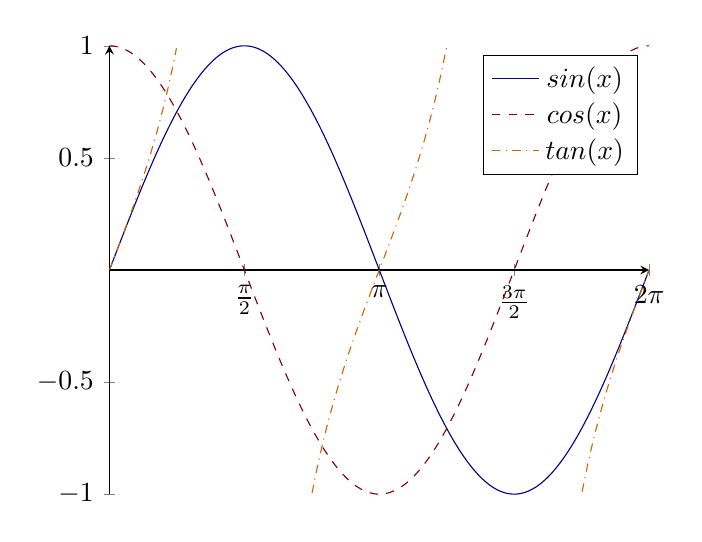
\begin{tikzpicture}
\begin{axis}[samples=1000,
	xtick={0,pi/2, pi, 3*pi/2, 2*pi},
	xticklabels={0, $\frac{\pi}{2}$,$\pi$, $\frac{3 \pi}{2}$, $2 \pi$,},
	ytick distance=0.5,
	restrict y to domain=-1:1,
	axis y line=center,
	axis x line=center,
	]
	\addplot[color=blue!50!black,domain=0:2*pi]{sin(deg(x))};
	\addlegendentry{\(sin(x)\)};
	\addplot[color=red!50!black, dashed, domain=0:2*pi]{cos(deg(x))};
	\addlegendentry{\(cos(x)\)};
	\addplot[color=orange!80!black, dashdotted, domain=0:2*pi]{tan(deg(x))};
	\addlegendentry{\(tan(x)\)};

\end{axis}
\end{tikzpicture}


Although immediately obscure, the shapes of these functions can be explained by
 imagining how the lengths of the different functions change as you rotate one 
revolution around the unit circle.







\end{document}
